\documentclass[a4paper,12pt]{article}

\usepackage[utf8]{inputenc}
\usepackage{geometry}

\geometry{
    left=1cm,
    right=1cm,
    top=1.5cm,
    bottom=2.5cm
}

\usepackage{setspace}
\usepackage{xcolor}
\usepackage{tikz}
\usetikzlibrary{trees}

\definecolor{lightblue}{RGB}{124, 214, 235}
\definecolor{middleblue}{RGB}{38, 150, 201}
\definecolor{darkblue}{RGB}{49, 86, 148}

\begin{document}

\pagenumbering{arabic}

\begin{Large}
    \begin{singlespace}
       \begin{center}
        \textbf{Stack - Template} \\
        Version 1.0.0
       \end{center} 
    \end{singlespace}
\end{Large}

\vspace*{10mm}

    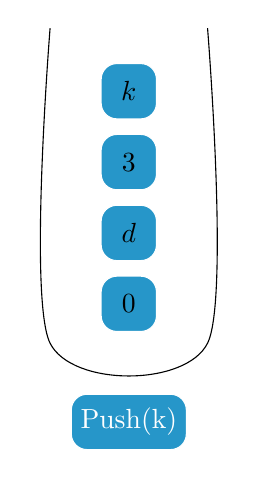
\begin{tikzpicture}[smooth, main/.style = {draw=white, text=black, fill=middleblue,  rounded corners=2mm, minimum size=2em}]
        \draw[x={(0cm,1cm)},y={(1cm,0cm)},color=black]
                plot coordinates{(4,1) (0,1) (0,3) (4,3)};
        \node[main] at (2, 0.5) {$0$};
        \node[main] at (2, 1.4) {$d$};
        \node[main] at (2, 2.3) {$3$};
        \node[main] at (2, 3.2) {$k$};
        \node[draw=white, text=white, fill=middleblue,  rounded corners=2mm, minimum size=2em] at (2, -1) {Push(k)};
    \end{tikzpicture}
    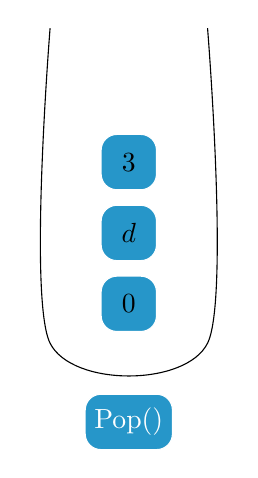
\begin{tikzpicture}[smooth, main/.style = {draw=white, text=black, fill=middleblue,  rounded corners=2mm, minimum size=2em}]
        \draw[x={(0cm,1cm)},y={(1cm,0cm)},color=black]
                plot coordinates{(4,1) (0,1) (0,3) (4,3)};
        \node[main] at (2, 0.5) {$0$};
        \node[main] at (2, 1.4) {$d$};
        \node[main] at (2, 2.3) {$3$};
        \node[draw=white, text=white, fill=middleblue,  rounded corners=2mm, minimum size=2em] at (2, -1) {Pop()};
    \end{tikzpicture}

\end{document}